\documentclass[twocolumn]{article}
\usepackage[utf8]{inputenc}
\usepackage[margin=0.8in]{geometry} %Margins
\usepackage{multicol} %Columns: multiples
\usepackage[hidelinks]{hyperref} %Hyperlinks
\usepackage{authblk} %Authors: affiliation
\renewcommand\Affilfont{\itshape\small} %Authors: affiliation font 
\usepackage{tabularx} % Tabular: automatic line-break
\usepackage[justification=raggedright]{caption} %Floats: caption as with tables
\usepackage{ltablex} %Floats: long
\renewcommand{\arraystretch}{1.5} %Tables: more space between rows 
\usepackage{graphicx} %Figures: import
\usepackage{subcaption} %Figures: multiple with one caption
\usepackage{amsmath} %Case definition
\usepackage[title]{appendix} %Appendix
\newenvironment{conditions} %Conditions
{\par\vspace{\abovedisplayskip}\noindent\begin{tabular}{>{$}l<{$} @{${}={}$} l}} %Conditions
{\end{tabular}\par\vspace{\belowdisplayskip}} %Conditions
\usepackage{natbib} %Citations: APA
\usepackage{amsmath} %Use \[ ... \] 
\usepackage{xcolor} %colors
\title{Aggregating food web nodes changes the keystone species of the network}
\author[1]{Emanuele Giacomuzzo}
\author[1,2]{Ferenc Jordàn}
\affil[1]{Balaton Limnological Institute, Centre for Ecological Research, Tihany, 8237, Hungary}
\affil[2]{Stazione Zoologica Anton Dohrn, Napoli, 80122, Italy}
\date{}
\begin{document}
\maketitle
\section*{Introduction}
    Trophic data management is something that ecologists always must deal with when working with food webs. Trophic interactions can be described among individuals, life stages, species, higher taxa, functional groups and several other, appropriately defined nodes of food webs. Some kind of aggregation is unavoidable, even the most highly resoluted food webs contain big aggregates (e.g., “bacteria'', see Martinez 1991). At the same time, even the least resoluted food webs may contain species (e.g., “hake”, see Yodzis 1998). Data aggregation can happen also during data analysis, especially in large networks, where the study of hundreds of nodes would be unfeasible \citep{Yodzis1999}.
    \par The way we decide to deal with data aggregation should consider the system we are modelling and the question we are trying to answer. Not taking this into consideration can bias the way by which we interpret the results of food web models (\citep{Paine1988, Hall1993}. For instance, various levels of aggregation at different trophic levels might bias our interpretation if we are trying to characterise the structure of a network \citep{Yodzis1999}. Both low- and high-resolution networks can be useful or useless, the key challenge is to properly match the problem, the data management, and the model construction. Even if this seems like a ubiquitous problem in food web ecology, standards for whether and how to aggregate data in a meaningful way does not exist yet. 
    \par The process of data aggregation assumes that there are nodes in the network that are similar enough that we can consider them the same node. For example, two fishes from the same genus might be aggregated into a node of the genus (e.g., Poecilia sphenops and Poecilia reticulata could be aggregated into Poecilia). To solve the problem of how to aggregate data, we need to define what we mean by similarity. 
    \par Similarity can be understood mathematically (equivalent network positions) and biologically (similar trophic habits). \citet{Yodzis1999} and \citet{Luczkovich2003} tried to answer this question by borrowing two definitions from social networks. \citet{Yodzis1999} borrowed the concept of structural equivalence – where two nodes are similar when sharing a high number of neighbours – and called the aggregation of structurally equivalent species” trophospecies”. \citet{Luczkovich2003} borrowed the concept of regular equivalence – where two nodes are similar when sharing a high number of similar neighbours, but not necessary the exact same – and said of nodes with high regular equivalence to have the same” trophic role”. 
    \par Another way by which we could think of species being similar is when they belong to the same food web module – in fact, aggregating the modules of a food web has been suggested already by \citet{Allesina2009a}. The two most reliable ways of finding modules in food webs are through the group model and modularity maximisation. The group model was firstly developed by \citet{Allesina2009a} and then extended by \citet{Sander2015}. Modularity maximisation was firstly applied to food webs by \citet{Guimera2010} following three definitions of modularity. The first one, which we will refer to as density-based modularity, is the degree by which nodes inside modules interact more among themselves than with nodes of other modules. The second one, which we will refer to as prey-based modularity, is the degree by which nodes inside modules tend to interact with the same predators. The third one, which we will refer to as predator-based modularity, is the degree by which nodes inside modules tend to interact with the same preys.
    \par In this paper, we investigate how these different aggregation methods maintain the relative importance of species, as a proxy of network structure. To compute the importance of species we used 15 of the most used centrality indices used in keystone species research. Our investigation was carried out on the data of the plankton food web of the Gulf of Naples (Figure 1), sampled at the Long-Term Ecological Research station MareChiara (LTER-MC) \citep{RiberadAlcala2004}). This is composed of 63 different nodes (see Table 1 of \citet{DAlelio2016} for the species assemblage). 
%    \begin{figure}[htbp]{\textwidth}
%        \centering
%        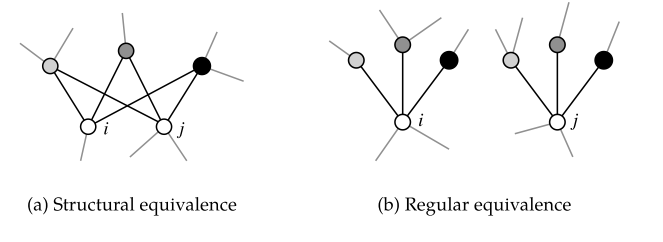
\includegraphics[width=.8\linewidth]{reg_struct_equivalence}
%        \caption{Two types of similarity indices highly used in social networks, which have been applied also to food webs.}
  %      \label{fig:equivalences}
  %  \end{figure}
\section*{Methods: clustering techniques}
    \subsection*{Hierarchical clustering of trophospecies}
        As a first clustering method, we clustered all the nodes belonging to the same trophospecies, as in \citet{Yodzis1999}. It was possible to find whether two nodes belong to the same trophospecies by calculating their similarity through the Jaccard similarity index. The clustering algorithm is as follows:
        \begin{enumerate}
            \item \emph{Compute similarity.} \smallskip \newline 
                Compute the similarity between the different nodes inside the food web. The Jaccard similarity can be calculated through the following equation \citep{Yodzis1999}
                    \begin{equation}
                        J_{ij}=\frac{a}{a+b+c}
                            \label{eqn:jaccard}
                    \end{equation}
                    where $J_{ij}$ is the Jaccard similarity between node i and j, a is the number of preys and predators that i and j have in common, b is the number of preys and predators of i, but not of j and c is the number of preys and predators of j, but not of i.
            \item \emph{Build the dendrogram.} \smallskip \newline 
                Find the two most similar elements\footnote{Elements are intended as nodes or clusters. Of course, during the first time we run this step all the elements are nodes. } and cluster them together\footnote{During our analysis, we used the function linkage of Matlab, which does not include the possibility of using a similarity matrix, so we converted the similarity matrices into dissimilarity ones. This was done by following what was written in \citet{VonLuxburg2004}. Namely, if the similarity function is normalised (takes values between 0 and 1) and always positive, then $d=1-s$ where d is the dissimilarity measure and s is the similarity measure.}. Repeat until you are left with only one item, which is the final dendrogram. During this process, the similarity between two clusters can be calculated in different ways, called linkage criteria. The ones that we used were
                \begin{itemize}
                    \item The similarity between the least similar nodes, one in each cluster, known as \textbf{single linkage} \citep{Frigui2008}
                    \item The similarity between the most similar nodes, one in each cluster, known as \textbf{complete linkage} \citep{Frigui2008}
                    \item The mean similarity between the nodes inside the first item and the second item, known as \textbf{weighted average distance(WPGMA)} \citep{Sokal1958}. See the following equation
                    \begin{equation}
                        d_{(i \bigcup j),k}=\frac{d_{i,k}+d_{j,k}}{2}
                            \label{eqn:WPGMA}
                    \end{equation}
                    \item The mean similarity between the nodes inside the first item and the second item, but taking into consideration the average distance between the items inside the fist cluster, known as \textbf{unweighted average distance (UPGMA)} \citep{Sokal1958}. See Equation 
                    \begin{equation}
                        d_{(i \bigcup j),k}=\frac{|i|d_{i,k}+|j|d_{j,k}}{|i|+|j|}
                            \label{eqn:UPGMA}
                    \end{equation}
                    where $d_{(i \bigcup j),k}$ is the distance between the cluster that includes i and j and k. $|i|$ and |$j$| are the mean distances between the elements inside i and j. 
                \end{itemize}
                A dendrogram was produced for every linkage criteria, then the dendrogram was selected by keeping the one with the highest cophenetic correlation \citep{Sokal1962}. This methods allows us to select between different linkage criteria the one that produces the dendrogram that preserves the most faithfully the pairwise dissimilarity between different elements. 
            \item \emph{Cut the dendrogram.} \smallskip \newline 
                Cut the dendrogram according to the maximum inconsistency of the branches. We used a threshold of 0.01. There is another method that you can use. This cuts the dendrogram by specifying what is the minimum similarity that two different species need to have to be part of the same cluster. This method, however, is more suitable if we have an arbitrary way of defining a cluster according to the similarity between its elements. By using this threshold, we can better find natural clusters arising from inside the data. 
            \end{enumerate}
    \subsection*{Hierarchical clustering of species according to their trophic role}
        As a second clustering method, we used hierarchical clustering to cluster nodes with similar trophic role, where the similarity between nodes is calculated by using the regular equivalence index (REGE), as in \citet{Luczkovich2003}. REGE can be calculated by using an algorithm of the same name, originally developed in the unpublished work by \citet{DouglasWhite1980,DouglasWhite1982,DouglasWhite1984} and was firstly described in the literature by \citet{Borgatti1993}. It is available to be used in the software of network analysis UCINET VI \citep{Borgatti2002}. The method wass exactly the same as the previous one, but this time the similarity between species was calculated through REGE instead of through the Jaccard index. The REGE index is calculated as follows \citep{Jordan2018}:
        \begin{enumerate}
            \item Set the number of iterations. We set 3 iterations. 
            \item Create the matrix $ R_{(t)} $, where t is the number of iterations. $     r_{(t)ij} $ is the regular equivalence between i and j at iteration t. Now set $ R_{(0)} $ as a matrix of ones. 
            \item Update the elements of the matrix following this sub-steps: 
            \begin{enumerate}
                \item For every predator k of species i, find the most similar predator m of     species j. Now, set $$ X_{i,k,j}=R_{km} $$ 
                \item For every predator m of species j, find the most similar predator k of     species i. Now, set $$ X_{j,m,i}=R_{mk} $$
                \item  For every prey h of species i, find the most similar prey n of species j. Now, set $$ Y_{i,h,j}=R_{hn} $$
                \item For every prey n of species j, find the most similar prey h of species i. Now, set $$ Y_{j,n,i}=R_{nh} $$ 
                \item Update the matrix R through Equation \ref{eqn:REGEupdate}. 
            \end{enumerate}
            \item Repeat the previous step for a number of iterations and let the regular equivalence matrix S be equal to the $ R_{t} $ . 
        \end{enumerate}
    \subsection*{Directed modularity (density based)}
        As a third clustering method, we found density-based clusters following the approach of \citet{Guimera2010}. The modularity of a directed network such as a food web, can be defined as the sum of the extra links present in a module relative to the number of links we would expect by knowing the indegree and outdegree of the nodes inside the module. Mathematically, it can be expressed as a generalisation of the Newman-Girvan modularity \citep{Newman2004} by using the following equation \citep{Arenas2007}
        \begin{equation}
            M_D(P)=\frac{1}{L}\sum\limits_{ij}[A_{ij}-\frac{k_i^{in}k_j^{out}}{L}]\delta_{m_im_j}
            \label{eqn:modularitydensity}
        \end{equation}
        \noindent where $M_D(P)$ is the directed modularity of partition P, $L$ is the number of links in the network, $A_{ij}$ is the element of the adjacency matrix of a directed, binary network (links go from $j$ to $i$), $k_i^{in}k_j^{out}/L$ is the probability of having an edge between $i$ and $j$, $k^{in}_i$ is the indegree of $i$ and $k^{out}_j$ is the out-degree of $j$), $ m_i$ is the module of $i$, and $\delta$ is the Kronecker delta. 
        \par By using the algorithm of spectral optimisation of \citet{Leicht2008} \footnote{an adaptation of the algorithm of \citet{Newman2006} for undirected networks}, we can find the number of modules and their node composition that maximises the modularity of the network. The algorithm goes as follows:
        \bigskip
        The point of the following steps is dividing the network into two modules and then keep diving these modules into other two modules so that every step maximises modularity.
        \begin{enumerate}
            \item \emph{Compute the modularity matrix} \smallskip \newline
            From the adjacency matrix (A), compute a matrix called the modularity matrix (B)
            \begin{equation}
                B_{ij}=A_{ij}-\frac{k_i^{in}k_j^{out}}{L} 
            \end{equation}
            and make it symmetric by transforming it into $B+B^T$ (this method of spectral optimisation requires the modularity matrix to be symmetric). 
            \item \emph{Find the eigenvector s} \smallskip \newline
            Find the eigenvector of the largest eigenvalue of $B+B^T$. We will call this eigenvector s.
            \item \emph{Calculate modularity} \smallskip \newline
            Calculate the modularity of the matrix through the following equation, which is a vectorised and symmetrised version of Equation \ref{eqn:modularitydensity} 
            \begin{equation}
                Q=\frac{1}{4m}s^T(B+B^T)s
            \end{equation}
            \item \emph{Finetune the vector s} \smallskip \newline
            Fine-tune the vector s by finding whether changing a single value would increase the modularity of the network. In case it does, change that value of the vector.
            \item \emph{Subdivide every module into two sub-modules} \smallskip \newline 
            Find the node segregation of the two newly created modules into two sub-modules that maximises modularity through step 2-4. Repeat until it is not possible to increase modularity by further subdivision.
        \end{enumerate}
    \subsection*{Directed modularity (pattern based)}
        As a fourth clustering method, we found pattern-based clusters following the approach of \citet{Guimera2010}. In this case, the modularity of a directed network is expressed as how much different nodes connect to the same neighbours. Mathematically, it can be expressed by the following equation \citep{Guimera2007}
        \begin{equation}
            M_O(P)=\sum\limits_{ij}[\frac{c_{ij}^{out}}{\sum\limits_lk_l^{in}(k_l^{in}-1)}-\frac{k_i^{out}k_j^{out}}{(\sum\limits_lk_l^{in})^2}]\delta_{m_im_j}
            \label{eqn:patternbasedmodularity}
        \end{equation}
        \noindent where $M_O(P)$ is the pattern-based modularity of the partition P, $c_{ij}^{out}$ is the number of outgoing links that i and j have in common, $k^{in}$ is the in-degree, $k^{out}$ is the out-degree, $\delta$ is the Kronecker delta and $m$ is the module of a certain species. 
        \par For simplicity, we used the spectral optimisation algorithm to maximise this type of modularity. Simulated annealing would have been a faster choice, but the two optimisation methods arrive to the same conclusion anyway \citet{Guimera2007}. The algorithm is the same exact as for the density-based modularity, but this time with the modularity matrix defined as
        \begin{equation}
            B_{ij} = 
            \begin{cases}
                \frac{c_{ij}^{out}}{\sum\limits_lk_l^{in}(k_l^{in}-1)}-\frac{k_i^{out}k_j^{out}}{(\sum\limits_lk_l^{in})^2}, & \mbox{if } i \neq j \\ 0 & \mbox{if } i=j 
            \end{cases}
        \end{equation} 
        % I need to take into consideration also same preys. I need to make a new function with preys instead of predators. 
    \subsection*{Group model}
        As a sixth clustering method, we clustered the nodes of every module that was found by the group model introduced by \citet{Allesina2009a}. This relies on considering the food web as a modular version of an Erdos-Renyi random graph \citep{Erdos1959} where the probability of having a link between two nodes depends upon which module they belong to. For an arbitrary number of modules k, the probability of generating the observed food web is 
        \begin{equation}
            P(N(S,L)|\vec{p}^{\,})=\prod_{i=1}^k\prod_{j=1}^k p_{ij}^{L_{ij}} (1-p_{ij})^{S_i S_j - L_{ij}}
        \end{equation}
        where $p_{ij}$ is the probability of a connection from a node of the group i to a node of the group j, $\vec{p}^{\,}$ is a vector containing all the probabilities $p_{ij}$, $L_{ij}$ is the number of links going from nodes of the group i to nodes of the group j, $S_i$ is the number of nodes in the group i and $S_j$ is the number of nodes in the group j. According to this model, we can recover the modular structure of a food web by finding the arrangement of nodes into modules that maximises this probability.
        \par This equation, however, cannot be solved analytically for each arrangement because of their high number - for example, a food web with 60 nodes produces more than $10^{59}$ arrangements. The algorithm of \citet{Sander2015} solves this problem by using a Metropolis-Coupled Markov Chain Monte Carlo ($MC^3$) (also known as parallel tempering) \citep{Geyer1991} using a Gibbs sampler \citep{Yildirim2012}.
\section*{Methods: wiring of the food web}
        \par We firstly created the binary version of the food web. To connected the clusters we invented a variation of the method of \citet{Martinez1991}: they used two methods to find links between different clusters, which they called the natural minimum cluster linkage (NMIN) and the natural maximum cluster linkage. For the NMIN, two clusters were connected to each other only if every node of the first cluster was connected to every node of the second cluster. For the NMX, two cluster were connected to each other if there was at least one link between a node of the first cluster and a node of the second cluster. They also used the 25\%, 50\% and 75\% of links. In our approach, we used used a range of percentages, spanning from 0,5\% to 100\% (with a growing rate of 0,5\%) and then we decided that the most adequate was going to be the one that maintain the structure of the network the best. This would have created different types of wiring - as well as different types of different food webs - according to what was the centrality index whose pattern we wanted to preserve. 
        \par Then we created the weighted version of the newly created food web. This was necessary because nwDC and STO consider the weight of the links between nodes. To do so, we used four different methods to calculate the weight between two clusters: we used the minimum weight between two nodes, one in each cluster, the maximum weight, the mean weight and the sum of the weights. 
        %By doing this, the resulting clustered network is just a binary one. Maybe this has biased my research. I need to add all the links together in the newly aggregated food web. 
\section*{Methods: centrality indices}
    \subsection*{Degree centrality (DC)}
        The degree centrality of a node ($DC$) describes how connected it is. It is the number of links a node has \citep{Wasserman1994} 
        \begin{equation}
            DC_i=\sum\limits_{j=1}^n A_{ij}    
        \end{equation}
        where $DC_i$ is the degree centrality of the node i, n is the number of nodes in the food web and $A_{ij}$ is the element of the adjacency matrix, after the network after has been transformed in a binary undirected one. It can be normalised by dividing it by the total number of possible connections that a node could have \citep{Wasserman1994} 
        \begin{equation}
            nDC_i=\frac{DC_i}{n-1}    
        \end{equation}
        where n is the number of nodes in the network. The minus arises from the fact that a species is not allowed to have a connection to itself (cannibalism in food webs).
        \par Another type of degree centrality that we considered was the weighted degree centrality (WDC), often referred to as node strength. Its formula, as well as the formula of its normalised version, are the same as for the non-weighted degree centrality. This time, however, the adjacency matrix is the the one of the undirected weighted network \citep{Fornito2016} 
        \begin{equation}
            WDC_i=\sum\limits_{j=1}^n A_{ij}
        \end{equation}
        \begin{equation}
            nWDC_i=\frac{WDC_i}{n-1}
        \end{equation}
    \subsection*{Closeness centrality (CC)}
        \indent The closeness centrality of a node (CC) describes how close it is to the other ones of the network. It is the average distance of a node from all other nodes and can be defined as \citep{Wasserman1994} 
        \begin{equation}
            CC_i=\frac{1}{\sum\limits_{j=1}^n d(i,j)}
        \end{equation} where d(i,j) is the distance between node i and j. It can be normalised as follows \citep{Wasserman1994}
        \begin{equation}
                nCC_i=\frac{n-1}{\sum\limits_{j=1}^n d(i,j)}
        \end{equation}
    \subsection*{Betweenness centrality (BC)}
        \indent The betweenness centrality (BC) describes how important a certain node is in the flow of energy through the network. It is the average number of times that a node acts a bridge along the shortest path between two other nodes, which is mathematically expressed as follows \citep{Wasserman1994} 
        \begin{equation}
            BC_i=\sum\limits_{i \neq m \neq n} \frac{\sigma_{mn}(i)}{\sigma_{mn}}
        \end{equation} where $\sigma_{mn}$ is the total number of shortest paths going from s to t and $\sigma_{mn}(i)$ is the total number of this paths passing through i. It can be normalised with the following equation \citep{Wasserman1994} 
        \begin{equation}
            nBC_i=\frac{BC_i}{(n-1)(n-2)/2}
        \end{equation} where n is the total number of nodes in the network.
    \subsection*{Status index (s)}
        The status index was firstly introduced to social networks, followed two years later by its application to food webs by \citet{Harary1959,Harary1961}. The status index of a node is the sum of its distances from all the other nodes inside the network, calculated as their shortest paths following a bottom-up direction \citep{Endredi2018}
        \begin{equation}
            s_i=\sum\limits^n_{j=1} d(i,j)
        \end{equation}
        where $s_i$ is the status index of species i, n is the total number of species inside the food web and $d(i,j)$ is the shortest path length between species i and species j. 
        \par There also two other indices related to it: the equivalent of the status index, but following a top-down direction (controstatus) 
         \begin{equation}
            s_i'=\sum\limits^n_{j=1} d(i,j)
        \end{equation}
        where $s_i$' is the controstatus of species i, and the difference between these two indices (net status)
        \begin{equation}
            \Delta s_i = s_i-s'_i    
        \end{equation}
        where $\Delta s_i$ is the net status of species i.
        
    \subsection*{Keystone index (K)}
        The keystone index was firstly introduced by \citet{Jordan1999} and inspired by the status index. 
        As the net status index, it is calculated by considering separately the bottom-up (like the status index), as well as the top-down (like the controstatus index) effects of a node \citep{Jordan2006}
        \begin{equation}
            K(i)=K_{b}(i)+K_{t}(i)
        \end{equation}
        where $K(i)$ is the keystone index of species i, $K_b(i)$ is its bottom-up keystone index and $K_t(i)$ is its top-down keystone index. 
        Unlike the status index, which only considers the distance between a node and all the other nodes, the keystone index takes into consideration how the magnitude of a certain effect gets split between the different neighbours of a node. Every time the effect reaches as certain node connected to multiple nodes, the following nodes receive only a fraction of the total effect. For example, when considering the bottom-up effect, if the prey has two predators, the bottom-up effect received by each predator will be half. 
        \par The bottom-up effect of a certain node $i$ is calculated in the following way
        \begin{equation}
            K_b(i)=\sum\limits_{j=1}^n\frac{1}{m(i)(j)}+\frac{K_b(j)}{m(i)(j)}
        \end{equation} where $j$ is a predator of $i$ and $m(i)(j)$ is the number of preys of $j$. $\frac{K_b(j)}{m(i)(j)}$ is the fraction of bottom-up effects of $j$ that are caused by $i$. The $K_b(j)$ of top-predators is set as 0. $K_t(i)$ is calculated exactly as $K_b(i)$, but this time by changing the direction of the links. 
        
        
        \par The keystone index is the sum of the bottom-up effects and the top-down effects, but also at the same time the sum of the direct and the indirect effects that a species has on its community %Expand on this 
        \begin{equation}
            K(i)=K_{dir}(i)+K_{indir}(i)
        \end{equation}
    \subsection*{Topological importance (TI)}
        The topological importance of a node represents its potential to create bottom-up effects on other species, up to a certain number of steps that we can set. It was firstly introduced to host-parasitoid networks by \citet{Muller1999} and then to food webs by \citet{Jordan2003}. The algorithm of its computation is as follows \citep{Jordan2009}:
        \begin{enumerate}
            \item \emph{Compute the one step matrix.} \smallskip \newline 
            In the one step matrix, if the energy flows from a prey to the predator, then the effect of the prey on the predator is the reciprocal of the indegree of the predator. For example, if the fox preys on mice, pigeons, beetles and shrews, the effect of mice on foxes would be $1/4$. 
            \begin{equation}
                a_{(1),ji}=in\:degree^{-1}_j
            \end{equation}
            \item \emph{Compute the n-step matrices.} \smallskip \newline 
            In the higher steps matrices, a node influences another node at a higher trophic level by summing the effects of every path that connects the two nodes. The effect of every path is the multiplication of the inverse of the outdegree of every node along the path. For a visual explanation see the Figure \ref{fig:TI}. 
%            \begin{figure}[htbp]{\textwidth}
   %             \centering
      %          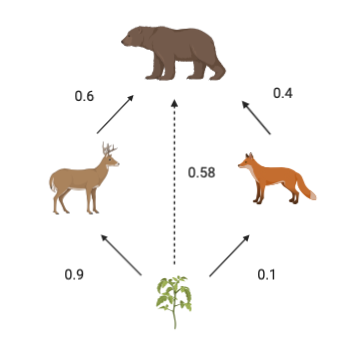
\includegraphics[width=.8\linewidth]{TI_example.png}
         %       \caption{Topological importance (TI) of a species on another. The effects of a prey on its predator are the sum of its effects along different paths. In this case, this plant species reaches the bear through two different paths. The first one is through the deer and the second is through the fox. The first path has an effect on the bear that is 0.9*0.6=0.54, the second one has an effect on the bear that is 0.1*0.4=0.04. Summing the effects through all the paths connecting the plant with the bear, we get the effect of the plant on the bear: 0.54+0.04=0.58. Figure created with BioRender.com.}
            %    \label{fig:TI}
            %\end{figure}
            \item \emph{Calculate topological importance} \smallskip \newline
            The topological importance of a node i ($TI_i$) can be calculated through the following formula
            \begin{equation} TI_i=\frac{\sum\limits^N_{m=1}\sum\limits^n_{j=1}a_{m,ji}}{N} \end{equation}
            where $N$ is the total number of steps considered, $m$ is the step number and $n$ is the total number of nodes in the network and $a_{m,ji}$ is the effect of species i on species j at m number of steps.    
        \end{enumerate}
        \par Topological importance can be also used for weighted networks, if instead of using the indegree we use the weighted degree \citep{Scotti2007}
        \begin{equation}
            a_{1,ji}=\frac{A_{ij}}{weighted\:indegree_j}
        \end{equation}
        where $A_{ij}$ is the element of the adjacency matrix of the weighted directed network. 
    \subsection*{Trophic field overlap (TO)}
        The trophic field overlap (TO) of a species represents how redundant its strong interactions are. It was firstly introduced by \citet{Jordan2009a}. It is the number of times that it and another node interact strongly with the same predator. The algorithm for its computation is as follows \citep{Jordan2018}
        \begin{enumerate}
            \item \emph{Compute the one-step matrix} \smallskip \newline 
            Compute the matrix telling us what is the effect of a species directly connected to another one. This is called the one-step matrix$ (A_{(1)}) $ and is calculated as 
            $$a_{(1)ij}=D_j^{-1}$$
            \par The difference with topological importance is that it consider the degree and not the indegree. 
            \item \emph{Compute the n-step matrix} \smallskip \newline 
            Compute the matrix telling us what is the effects of a species connected to another one through other species. This is called the n-step matrix$ (A_{(n)}) $ and can be calculated as follows: $$A_{(n)}=A_{(1)}^n$$
            \item \emph{Compute the average effect matrix} \smallskip \newline
            Compute the effect a species has on another species averaged by the number of steps in the average effect matrix $(E_{(n)})$
            \begin{equation}
                E_n=\frac{1}{n}\sum\limits^n_{i=1}A_{(i)}
            \end{equation}
            \item \emph{Compute the interactor matrix} \smallskip \newline 
            Compute a matrix whose values tell us whether the interaction between two species is strong or not. This is called the interactor matrix $ (M_T) $. To do this, we need to define a threshold over which a certain interaction is considered to be strong. The elements of the interactor matrix are S if the interaction is strong and W if the interaction is weak. 
            \item \emph{Compute the topological overlap matrix} \smallskip \newline 
            Compute a matrix with how many times two species interact strongly with the same predator. This is called the topological overlap matrix.
            \item \emph{Compute TO} \smallskip \newline 
            Calculate the topological overlap of species. This is the sum of how many times other species interact strongly with its same predator. It can be calculated by summing the elements of the rows of the topological overlap matrix.
        \end{enumerate}
        \par Trophic overlap can also be calculated by taking into account the interaction strength between nodes by constructing the one-step matrix in the following way \citep{Xiao2019}
        \begin{equation}
            a_{(1)ij}=\frac{W_{ij}}{WD_j}    
        \end{equation}
        where $W_{ij}$ is the proportion of i in the diet of j or vice versa (the network is undirected), taking into consideration interaction strength, and $WD_j$ is the weighted degree of j (the sum of all its interaction strengths). %???
        \par Finally, to avoid the bias of choosing a wrong threshold, we chose multiple thresholds and summed the TO of a species i for each of these thresholds. This gave us the species uniqueness (STO), an index that was firstly introduced by \citet{Lai2015}. 
    \subsection*{Trophic position (TP)}
        Trophic position is an adaptation of trophic level to include cycles and fractional positions and was firstly introduced by \citet{Levine1980}. It is the mean path length energy flows from the autotrophs to a certain species. The trophic position of a certain species ($TP_i$) can be calculated as
        \begin{equation}
            TP_i=\sum\limits_{k=0}^\infty k \cdot p_i(k).
        \end{equation}
        where k is a certain path length and $p_i(k)$ is the probability that species i will reach the energy produced by the autotrophs via a path of length k.
\section*{Methods: wiring of the food web and statistical analysis}
    The clusters were then connected following a similar approach to the one of Martinez (1991) – two clusters were connected only if a certain percentage of links between their nodes was realised. In our work, we used different percentages going from 1\% to 100\% with a growing rate of 1\%.  Then we found the weight of these links by using four different methods. By looking at the links between the nodes of the first and the second cluster, we considered their minimum weight, their maximum weight, their mean weight and the sum of the weights as the weight of the link between the two clusters. Then, we calculated the centrality indices for all these newly created food webs. Then we calculated the centrality index for every newly created food web. For each centrality index, we kept the food web that maintained the best the rank of the original species. 
    \par To see how the new food web maintained the best rank of the original species with compared the centrality index of the nodes before the clustering and wiring and after, through the intraclass correlation coefficient (ICC). ICC estimates and their 95\% confident intervals were calculated using the Matlab function Intraclass Correlation Coefficient (ICC) \citep{Salarian2021} based on a single-rating, consistency, 2-way mixed-effects model (see \citet{McGraw1996}).  This is also known as norm-referenced reliability or as Winer's adjustment for anchor points \citep{Winer1971}.
    This allowed us to select the link percentage and the interaction strength method that maintained the ranking the best.
\section*{Results}
    \subsection{Clustering}
        The result of clustering gave 39 cluster for the Jaccard index hierarchical clustering, 14 clusters for the REGE index hierarchical clustering, 13 clusters for the pattern modularity, 11 clusters for the density modularity and 8 for the group model.
        The species that were unique inside their module were for Jaccard index -> 14,9,33,7,30,21, and others.
    \subsection{Food web wiring}
        The best link percentage, interestingly enough, was the lowest, 0.5\%. It seems like then that it is better to use NMIN than NMAX. This seems also like that the way we should wire a food web doesn't have trade-offs between preserving different types of features of the food web represented by the centrality indices. The result of the five food webs is the following one in Figure \ref{}. 
        \par We found linking the clusters through the minimum method giving poor results in this case. Many clusters had a weight < 0.0001, which rounded the connection between clusters to 0, loosing all the structure of the food web.  
        %I need to find a good way of representing the food webs where species have different colors. 
    \subsection{Centrality indices}
        It seems like Jaccard maintains the bottom-up effects slightly better than REGE and REGE maintain the top-down effects slightly better than Jaccard. It is interesting because it seems like REGE and Jaccard maintain the structure of the food web in a similar way, but they give a really different number of clusters. I am wondering if the Jaccard groups are nested inside the REGE groups. We could say that both of the methods are fair methods for clustering. Jaccard could be used for clustering food webs when we are interested only in a particular one, meanwhile REGE could be used to study the same node in different food webs, as suggested by \citet{Luczkovich2003}. It is not a surprise that the density modularity doesn't maintain the structure. This is because it tends to find species that form sub communities of interacting species, more than species who show the same type of predator and prey. However, it is surprising to us that pattern modularity is not best algorithm. This is because we thought that it would have used the maximum power of algorithms to find the species that connect to the same predator. This might have been the problem: it aggregates species with the same predator, but not with the same prey.
        Watch out: the node number 59 was not connected to anything, so it has been deleted. See Figure \ref{fig:heatmap}.
%        \begin{figure*}
%            \centering
%            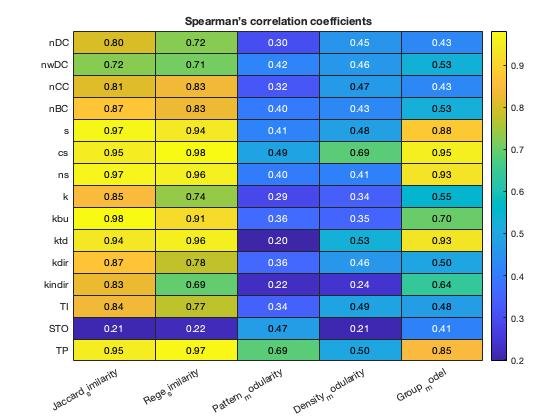
\includegraphics[width=1\linewidth]{results.jpg}
%            \caption{Heat map of how different methods of clustering preserve the relative importance of species inside the food web of the Gulf of Naples. The values represent the Kendall's coefficient of concordance     (Kendall's W). In the next figure I will tell you which ones were the ones that seemed to preserve the pattern.}
%            \label{fig:heatmap}
%pdflatex        \end{figure*}
\section*{Discussion}
    A possible future direction is using new algorithms for clustering. These could be either hierarchical clustering with different types of similarity indices - such as automorphic equivalence \citep{Wasserman1994} or Katz similarity \citep{Newman2018} - or methods of directed network clusterings. For the latter type of clustering, check out the excellent review of \citet{Malliaros2013}. Some examples of these algorithms are the semi-supervised learning \citep{Zhou2005}, the two-step random walk \citep{Huang2006}, the mixture models \citep{Newman2007,Ramasco2008,Wang2008}, the infomap \citep{Rosvall2008}, the Link Rank algorithm \citep{Kim2010} and the maga method \citep{Zhan2011}. \citet{Zhou2005,Huang2006,Wang2008,Kim2010} and \citet{Zhan2011} have never been cited by the ecological literature and their application to food webs might reveal to be useful. 
    \par Another possible direction is checking how different data aggregations influence the dynamics and not only the structure of the network. 
    \par The repercussion of food web aggregation on sampling have been also investigated by \citet{Patonai2017}.
    Considering that it would be difficult to know in advance what would be the connections between different species in the food web (I mean, we can kind of know, but not exactly I guess. Actually in some cases we can, so it is no problem. But in other cases it might be more difficult). A good future direction would be trying to understand when do species have the same trophic role. What is the biology behind this? Can we predict by using functional traits what are the species that have the same trophic role? 
    \par Also it needs to test to what extent are centrality indices a good proxy for food web structure. 
    \par I think that it is really important for a certain aggregation method to maintain the trophic position of the different species. This is because the trophic level of a species is associated with many information about its role inside a food web. Trophic level is a proxy for many things. %Read about this.
    I think that if a method doesn't maintain the trophic level of a species, it can't be a reliable one for maintaining the structure of the network. 
    \par It is also important to remember that it seems like species who are unique trophospecies seem to be really important for secondary extinction. In particular, \citep{Petchey2008a} found that they are particularly vulnerable to secondary extinctions when trying to model their dynamic food web. The fact that the concept of trophospecies not only is important to understand which ones are the most vulnerable species in the system, but it seems also important in something related to how different species are related to each other. If, as someone said but I don't remember who, keystone species are the ones that are unique in their trophospecies, it means that secondary extinctions happen only if you hit the network close or on keystone species. This is because keystone species, if my interpretation is correct, are not only the most important, but also the most vulnerable. This might be due to the fact that they have such low abundance as well. %Who said that keystone species emerge when you can aggregate the network?
    So, at this point, maybe data aggregation would reveal keystone species. The fact that the aggregation of according to Jaccard not only can reveal the keystone species, but also would maintain the relative importance of the nodes, seems like a great way of aggregating data. Wait: I need to check whether the species that are unique in their cluster also have high centrality indices.  
    \par A problem is always the one from the fact that food webs are more resolved at higher than at lower trophic levels. For example, a node at the highest trophic level might represent a single species of shark, meanwhile a node at the bottom trophic level might represent hundreds of phytoplankton species \citep{}.
    \par Understanding how to aggregate data might also help us with dealing with missing data. 
    \par We would not suggest to use modularity maximisation and the group model for data aggregation.
    \par One of the things that needs to be defined as well is: what is the relevance of the clusterings at this point? 
    \par For my networks maybe I should have also networks that are really different between each other in terms of size and in terms of habitat. 
    %What are the parameters of the network that I should estimate? I think connectance would be a good one because it is important in the niche model.
    
\section*{Acknowledgments}
    We would like to thank Domenico D'Alelio %him or someone else? 
    for the data-set of the food web of the Gulf of Naples, Wei-chung Liu for providing the code for computing some of the centrality indices (keystone index, topological importance and trophic level) and Stefano Allesina \& Elizabeth Sander for providing the code for the  computation of the group model. 
\section*{Supplementary material}
    The adjacency matrix of the food web of the Gulf of Naples, as well as the code used to analyse it is available at \url{https://github.com/Emanuele-Giacomuzzo/Data_aggregation}. This research resulted also in the creation of the Matlab toolbox "Food Web Tools" available at  \url{https://uk.mathworks.com/matlabcentral/fileexchange/food-web-tools}. It is necessary to install it to be able to run the code available in Github.
\bibliographystyle{apalike}
\bibliography{library}
\begin{appendices}
    \section*{Equations}
        \begin{equation}
            R_{(t)ij}=\frac{\sum\limits_{k=1}^?{X_{i,k,j}}+\sum\limits_{m=1}^?{X_{j,m,i}}+\sum\limits_{h=1}^?{Y_{i,h,j}}+\sum\limits_{n=1}^?{Y_{j,n,i}}}{MAX(\sum\limits_{k=1}^?{X_{i,k,j}}+\sum\limits_{m=1}^?{X_{j,m,i}}+\sum\limits_{h=1}^?{Y_{i,h,j}}+\sum\limits_{n=1}^?{Y_{j,n,i}})}
                \label{eqn:REGEupdate}
        \end{equation}
\end{appendices}
\end{document}